\chapter{Modélisation UML du Smart WMS}
\label{chap:uml}

% Large UML diagrams are deliberately split into two readable portrait views.
\newcommand{\umlpair}[4]{%
\begin{figure}[p]
\centering
\includegraphics[width=.98\linewidth,height=.76\textheight,keepaspectratio]{#1}
\caption{#3 (partie 1 sur 2).}
\label{#4}
\end{figure}
\begin{figure}[p]
\centering
\includegraphics[width=.98\linewidth,height=.76\textheight,keepaspectratio]{#2}
\caption*{\textbf{Suite de la figure \ref{#4}.} #3 (partie 2 sur 2).}
\end{figure}
\FloatBarrier
}
\newcommand{\umlquad}[6]{%
\begin{figure}[p]\centering
\includegraphics[width=.96\linewidth,height=.77\textheight,keepaspectratio]{#1}
\caption{#5 (partie 1 sur 4).}\label{#6}
\end{figure}
\begin{figure}[p]\centering
\includegraphics[width=.96\linewidth,height=.77\textheight,keepaspectratio]{#2}
\caption*{\textbf{Suite de la figure \ref{#6}.} #5 (partie 2 sur 4).}
\end{figure}
\begin{figure}[p]\centering
\includegraphics[width=.96\linewidth,height=.77\textheight,keepaspectratio]{#3}
\caption*{\textbf{Suite de la figure \ref{#6}.} #5 (partie 3 sur 4).}
\end{figure}
\begin{figure}[p]\centering
\includegraphics[width=.96\linewidth,height=.77\textheight,keepaspectratio]{#4}
\caption*{\textbf{Suite de la figure \ref{#6}.} #5 (partie 4 sur 4).}
\end{figure}
\FloatBarrier
}
\makeatletter
\setlength{\@fptop}{10pt}
\setlength{\@fpbot}{0pt plus 1fil}
\makeatother

\section{Objectifs et démarche de modélisation}
\label{sec:5.1}

L'architecture fonctionnelle du chapitre précédent décrit les responsabilités attendues du Smart WMS. La modélisation UML complète cette vue en précisant les acteurs, les enchaînements métier, les échanges entre systèmes et les objets manipulés. Elle ne remplace pas l'architecture fonctionnelle : elle la rend vérifiable à différents niveaux de lecture.

La démarche part des cas d'utilisation identifiés au chapitre~3. Les diagrammes de cas d'utilisation répondent à la question «~quoi et pour qui~?~». Les diagrammes d'activité décrivent le déroulement des processus. Les diagrammes de séquence précisent les interactions entre les acteurs, le WMS et les systèmes externes. Enfin, le modèle de domaine et le diagramme de composants donnent une vue stable des objets métier et de l'organisation logique de la solution.

La classification 	extit{Core / Smart / Optional} est conservée dans l'ensemble des vues. Une capacité 	extit{Core} est nécessaire au fonctionnement courant. Une capacité 	extit{Smart} améliore une décision lorsque les données sont suffisantes. Une capacité 	extit{Optional} dépend d'un équipement ou d'un système particulier. Cette séparation évite de présenter une technologie comme une condition préalable à un processus métier fondamental.

\section{Modélisation des cas d'utilisation}
\label{sec:5.2}

Les cas d'utilisation traduisent les besoins en interactions observables entre les acteurs et le système. La relation \emph{include} est utilisée lorsqu'un comportement fait partie du traitement principal ; la relation \emph{extend} est réservée à une situation conditionnelle, par exemple une anomalie ou l'utilisation d'un dispositif de vision. Les relations ne sont donc pas multipliées lorsqu'elles n'apportent pas de clarification.

\subsection{Vue globale}
\label{sec:5.2.1}

La vue globale regroupe les grands domaines sans reproduire les dizaines de cas détaillés. Elle met en évidence le rôle des opérateurs, responsables, planificateurs et systèmes externes dans les domaines métier, les services de support et l'aide à la décision.

\begin{figure}[p]\centering
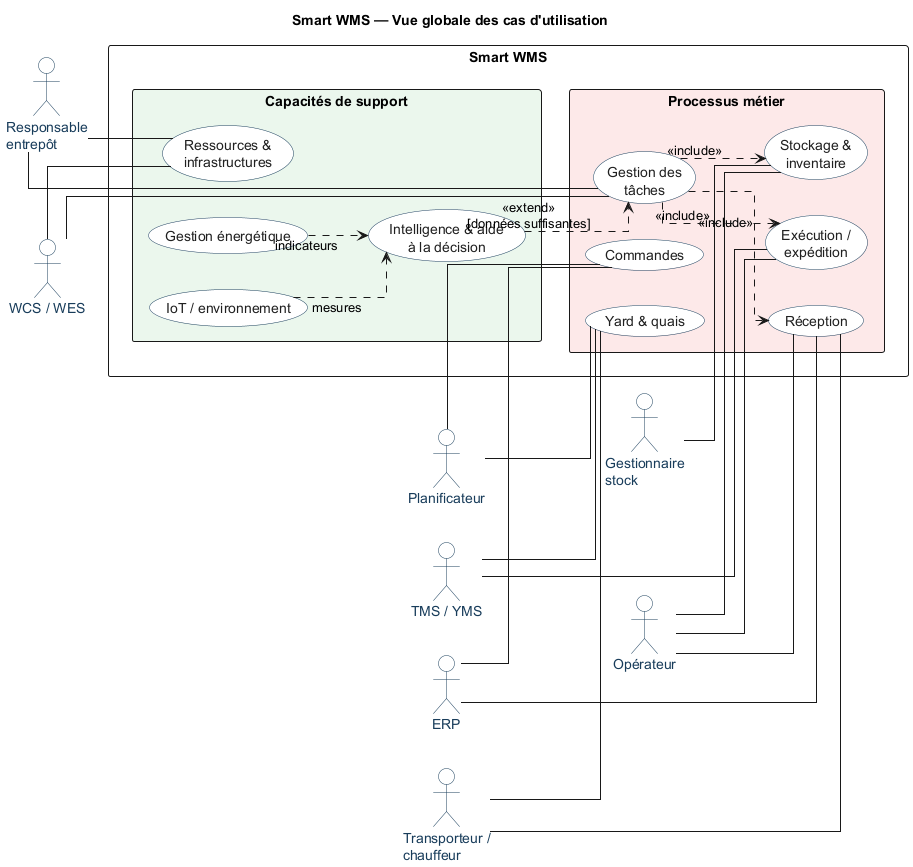
\includegraphics[width=.92\linewidth,height=.78\textheight,keepaspectratio]{figures/uml/uc_global.png}
\caption{Vue globale des cas d'utilisation du Smart WMS.}\label{fig:uc-global}
\end{figure}\FloatBarrier

\subsection{Réception}
\label{sec:5.2.2}

La réception couvre la planification du rendez-vous, la réception physique, l'identification et les contrôles avant la proposition d'emplacement. Les cas UC-R01 à UC-R07 constituent le socle opérationnel. UC-R08 apporte une prévision de charge. UC-R09 à UC-R12 ne sont activés que si les équipements ou les données nécessaires sont disponibles.

\begin{figure}[p]\centering
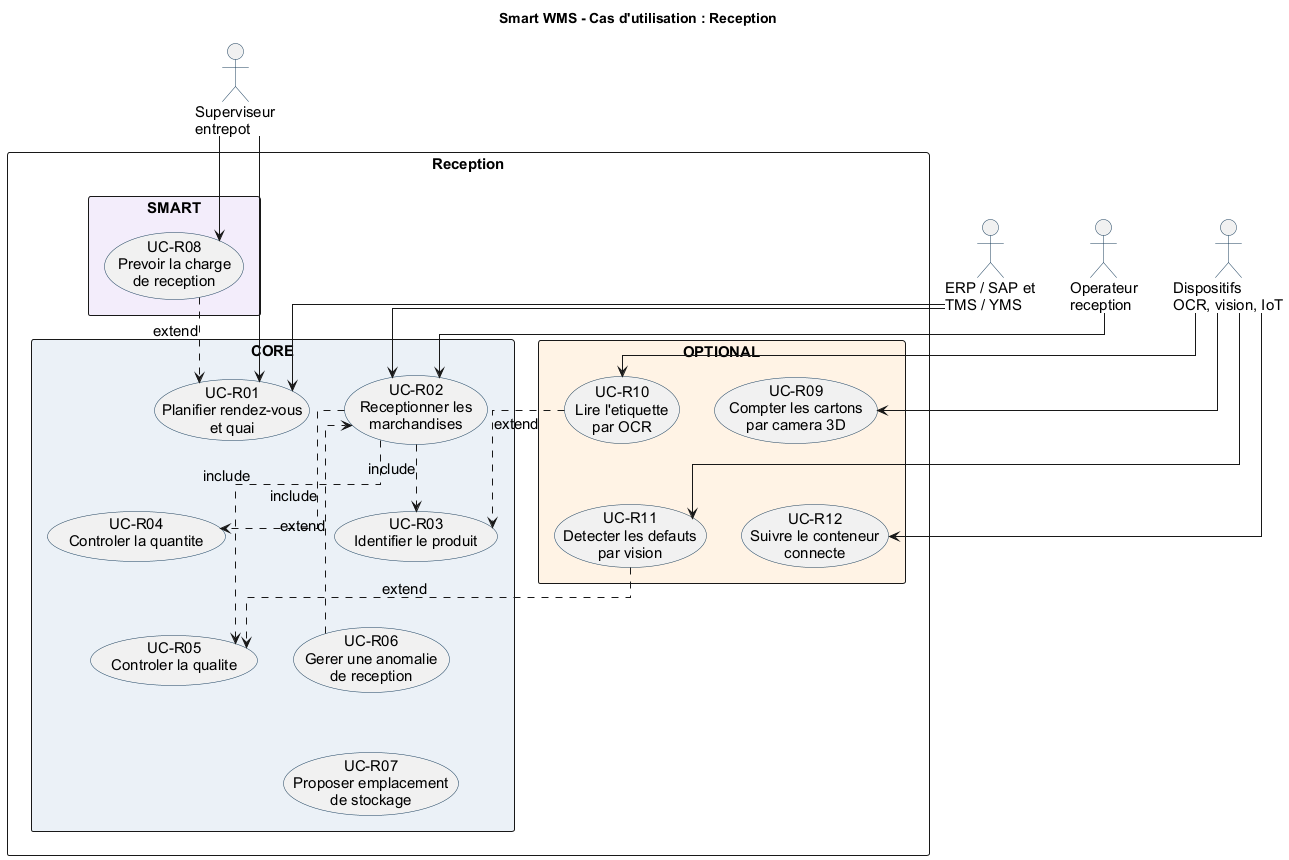
\includegraphics[width=.92\linewidth,height=.78\textheight,keepaspectratio]{figures/uml/uc_reception_portrait.png}
\caption{Cas d'utilisation de la réception : UC-R01 à UC-R12.}\label{fig:uc-reception}
\end{figure}\FloatBarrier

\subsection{Stockage et inventaire}
\label{sec:5.2.3}

Le modèle de stockage distingue les opérations de mise en stock, de suivi des stocks, d'emplacements, de lots et d'inventaire des capacités d'optimisation ou de prédiction. Le slotting et la prévention des ruptures sont des capacités 	extit{Smart}; le RFID et les AMR/AGV restent des options dépendantes de l'infrastructure.

\begin{figure}[p]\centering
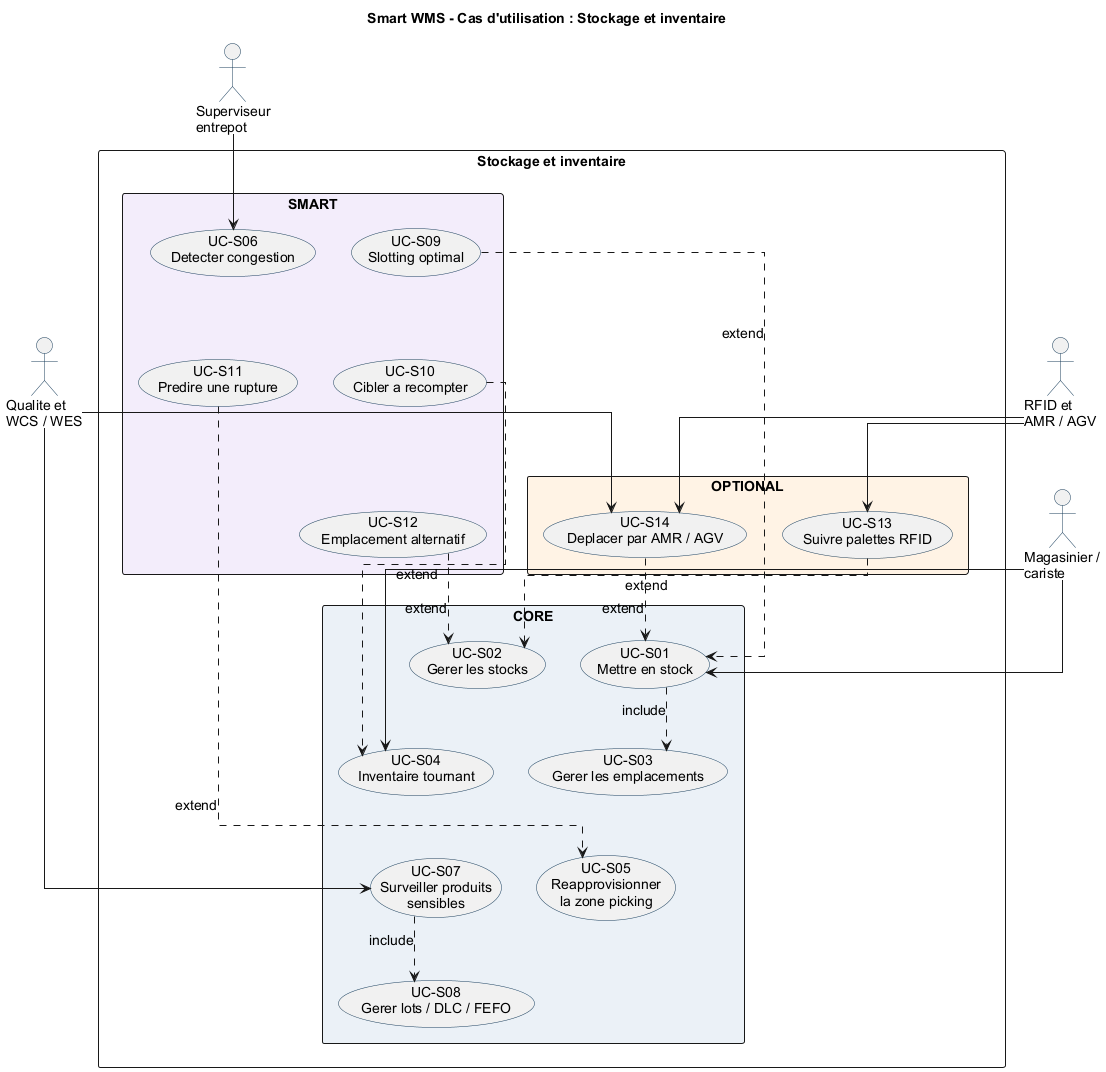
\includegraphics[width=.90\linewidth,height=.79\textheight,keepaspectratio]{figures/uml/uc_stockage_portrait.png}
\caption{Cas d'utilisation du stockage et de l'inventaire : UC-S01 à UC-S14.}\label{fig:uc-stockage}
\end{figure}\FloatBarrier

\subsection{Commandes, exécution et expédition}
\label{sec:5.2.4}

Cette vue rassemble les cas UC-E01 à UC-E15 définis au chapitre~3, depuis l'ordonnancement jusqu'à la confirmation d'expédition et au traitement des retours. Les optimisations de vagues, de parcours et de charge complètent le processus sans se substituer à l'exécution WMS.

\begin{figure}[p]\centering
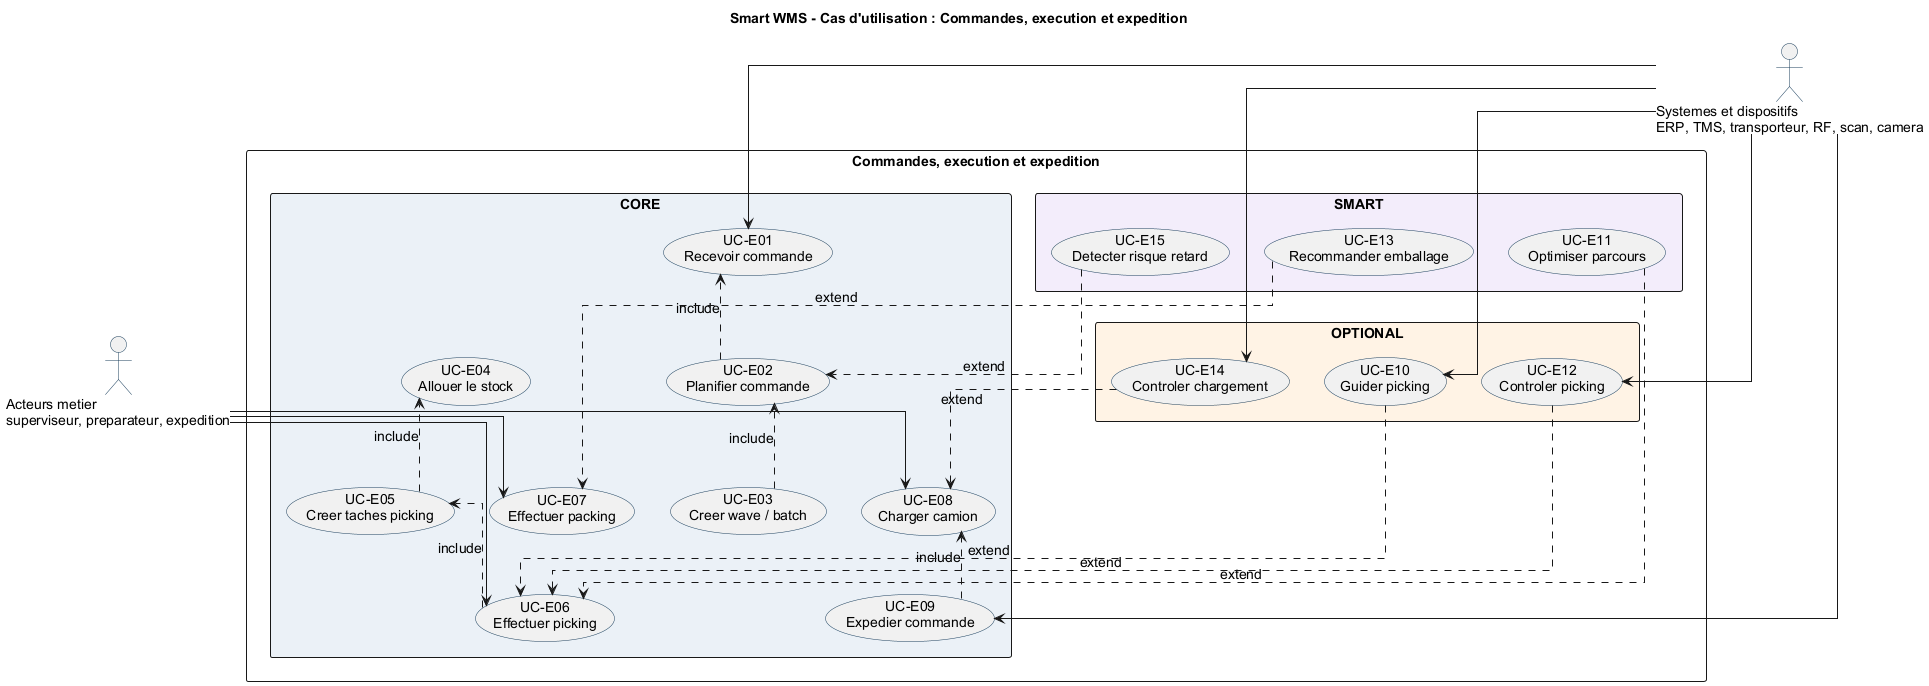
\includegraphics[width=.92\linewidth,height=.79\textheight,keepaspectratio]{figures/uml/uc_expedition_portrait.png}
\caption{Cas d'utilisation des commandes, de l'exécution et de l'expédition : UC-E01 à UC-E15.}\label{fig:uc-expedition}
\end{figure}\FloatBarrier

\subsection{Yard, quais et ressources}
\label{sec:5.2.5}

La gestion de la cour et des quais formalise les cas UC-Y01 à UC-Y07. La gestion des ressources et infrastructures regroupe les cas UC-RES01 à UC-RES10 relatifs au personnel, aux équipements, aux actifs, à l'énergie et aux interfaces WCS/WES. Les deux domaines restent distincts : le premier pilote les flux de véhicules et de quais, le second décrit les moyens disponibles pour les exécuter.

\begin{figure}[p]
\centering
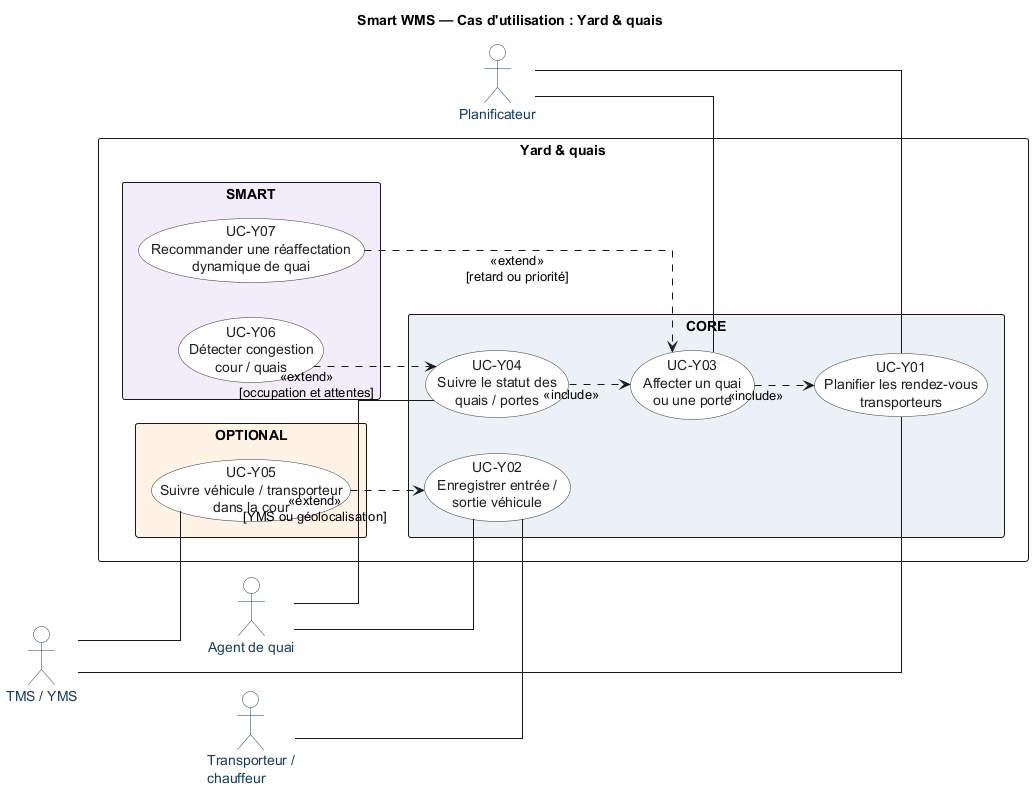
\includegraphics[width=.96\linewidth,height=.70\textheight,keepaspectratio]{figures/uml/uc_yard.png}
\caption{Cas d'utilisation de la gestion du yard et des quais : UC-Y01 à UC-Y07.}
\label{fig:uc-yard}
\end{figure}

\begin{figure}[p]
\centering
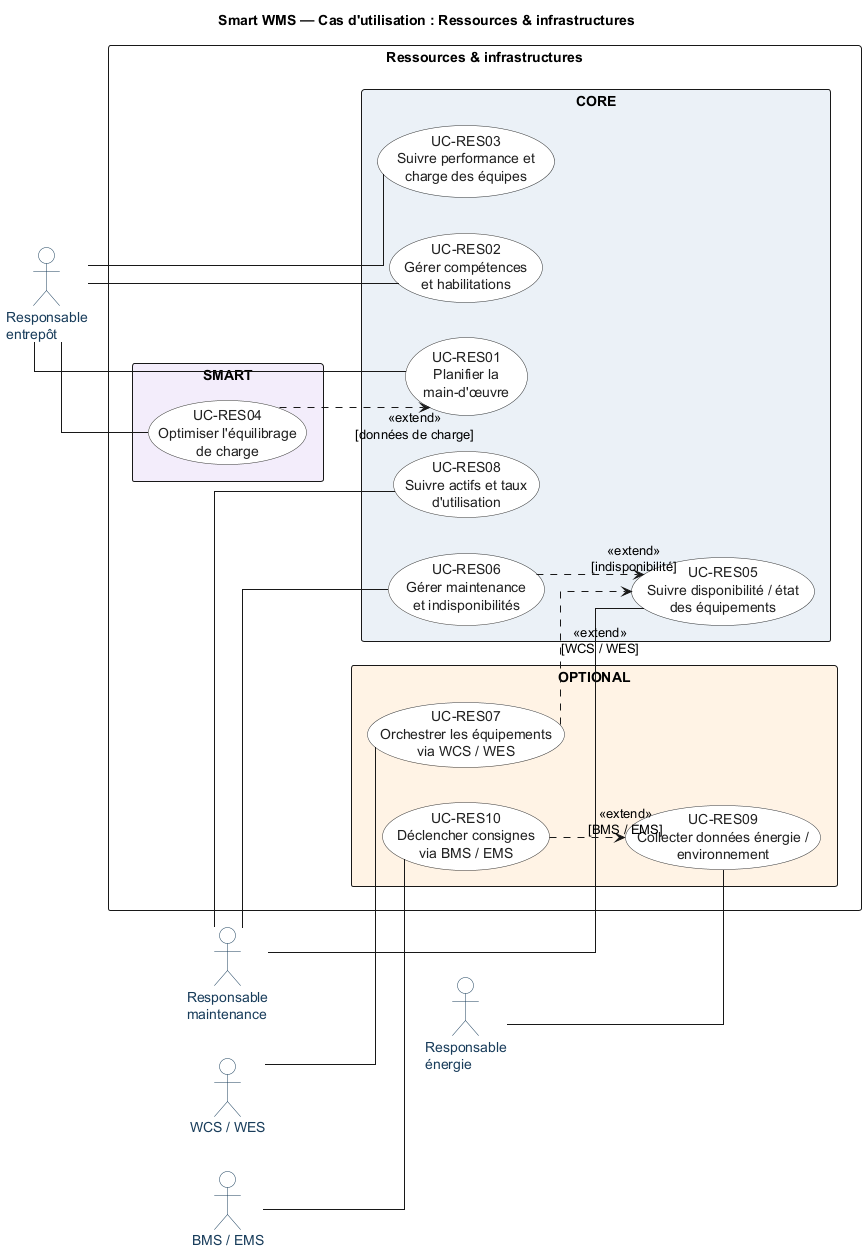
\includegraphics[width=.96\linewidth,height=.78\textheight,keepaspectratio]{figures/uml/uc_ressources.png}
\caption{Cas d'utilisation des ressources et infrastructures : UC-RES01 à UC-RES10.}
\label{fig:uc-ressources}
\end{figure}
\FloatBarrier

\subsection{Capacités intelligentes transversales}
\label{sec:5.2.6}

Les fonctions transversales exploitent les données issues des processus sans recréer ces processus. Elles couvrent la prévision, l'optimisation, la détection d'anomalies, les recommandations, l'environnement et l'énergie. Une recommandation doit toujours être rattachée à une règle, à une donnée observable et à une décision métier contrôlable.

\begin{figure}[p]\centering
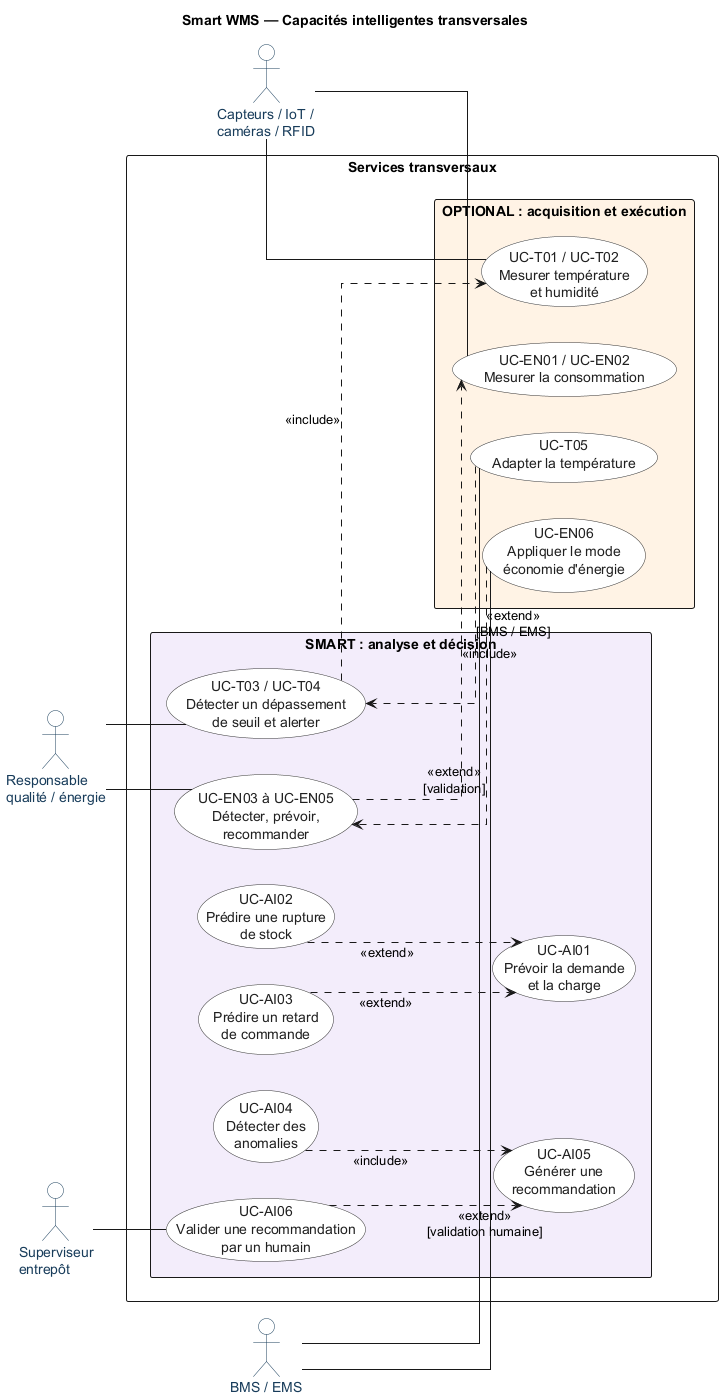
\includegraphics[width=.94\linewidth,height=.78\textheight,keepaspectratio]{figures/uml/uc_transversal.png}
\caption{Capacités intelligentes et infrastructurelles transversales du Smart WMS.}\label{fig:uc-transversal}
\end{figure}\FloatBarrier

\section{Modélisation des processus métier}
\label{sec:5.3}

Les diagrammes d'activité montrent les décisions qui structurent les processus. Ils distinguent les contrôles obligatoires des traitements conditionnels et rendent visibles les points où une information, une validation ou une exception modifie le parcours.

\subsection{Réception et mise en stock}

Le processus de réception enchaîne le rendez-vous, la réception, l'identification, les contrôles et le traitement éventuel des anomalies. La mise en stock est ensuite déclenchée avec un emplacement conforme aux contraintes du produit et de l'entrepôt.

\begin{figure}[p]
\centering
\includegraphics[width=.90\linewidth,height=.84\textheight,keepaspectratio]{figures/uml-source/DA_reception.png}
\caption{Diagramme d'activité du processus de réception.}
\label{fig:activity-reception}
\end{figure}
\FloatBarrier

\subsection{Stockage et exécution des commandes}

Le stockage combine la décision de mise en stock, le contrôle des contraintes et la mise à jour de l'inventaire. Le processus aval organise quant à lui la préparation, le contrôle et la confirmation de l'expédition. Les étapes d'optimisation restent conditionnées par les données et les règles applicables.

\begin{figure}[p]
\centering
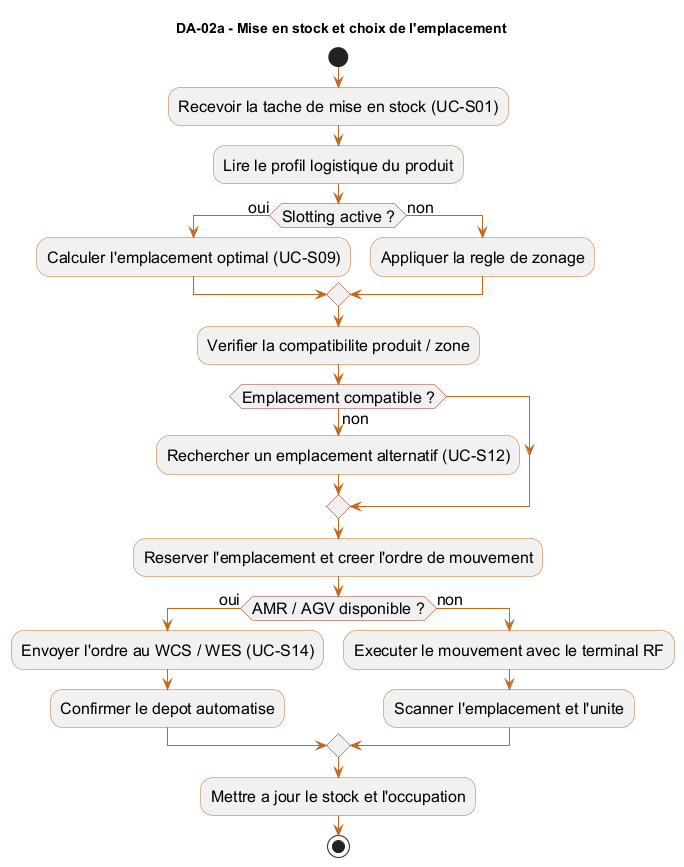
\includegraphics[width=.82\linewidth,height=.77\textheight,keepaspectratio]{figures/uml/activity_stockage_putaway.png}
\caption{Diagramme d'activité de la mise en stock et du choix d'emplacement.}
\label{fig:activity-stockage-putaway}
\end{figure}
\clearpage
\begin{figure}[p]
\centering
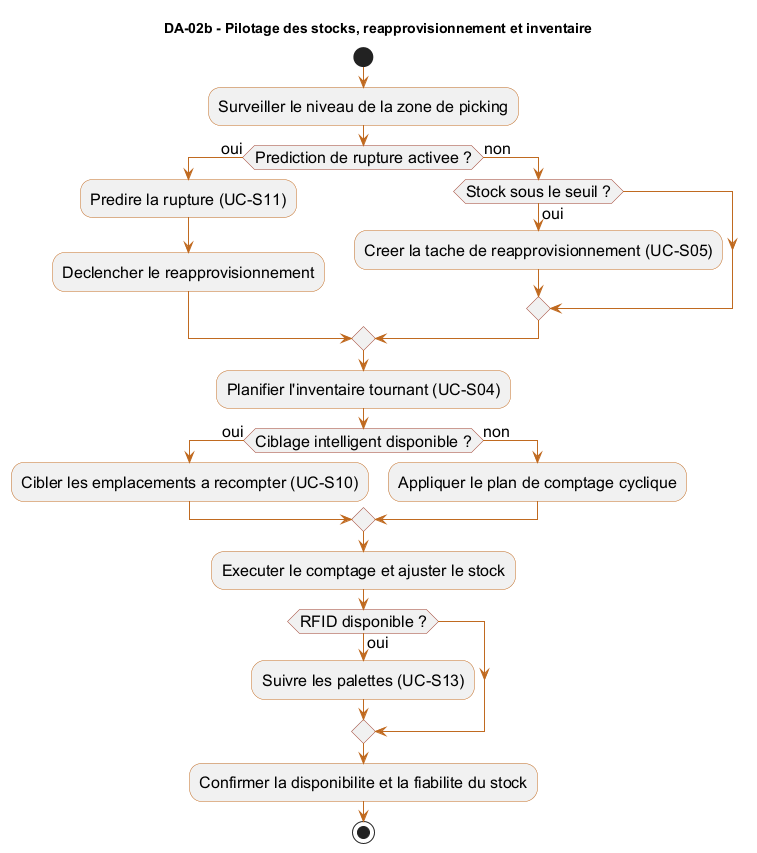
\includegraphics[width=.82\linewidth,height=.77\textheight,keepaspectratio]{figures/uml/activity_stockage_pilotage.png}
\caption{Diagramme d'activité du pilotage des stocks, du réapprovisionnement et de l'inventaire.}
\label{fig:activity-stockage}
\end{figure}
\FloatBarrier

\begin{figure}[p]
\centering
\includegraphics[width=.90\linewidth,height=.84\textheight,keepaspectratio]{figures/uml-source/DA_expedition.png}
\caption{Diagramme d'activité du processus de préparation et d'expédition.}
\label{fig:activity-expedition}
\end{figure}
\FloatBarrier

\section{Interactions entre acteurs et systèmes}
\label{sec:5.4}

Les séquences complètent les activités en rendant explicites les messages échangés. La réception illustre la synchronisation avec l'ERP et l'utilisation contrôlée de moyens de capture. L'expédition montre l'interaction entre le WMS, le terminal opérateur, le TMS/YMS et les services d'optimisation.

\begin{figure}[p]
\centering
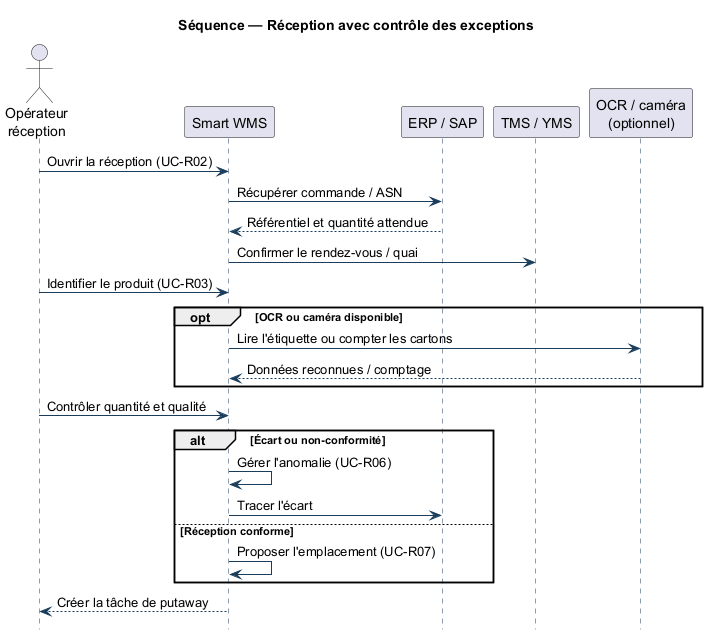
\includegraphics[width=.96\linewidth,height=.78\textheight,keepaspectratio]{figures/uml/seq_reception.png}
\caption{Diagramme de séquence de la réception.}
\label{fig:sequence-reception}
\end{figure}

\begin{figure}[p]
\centering
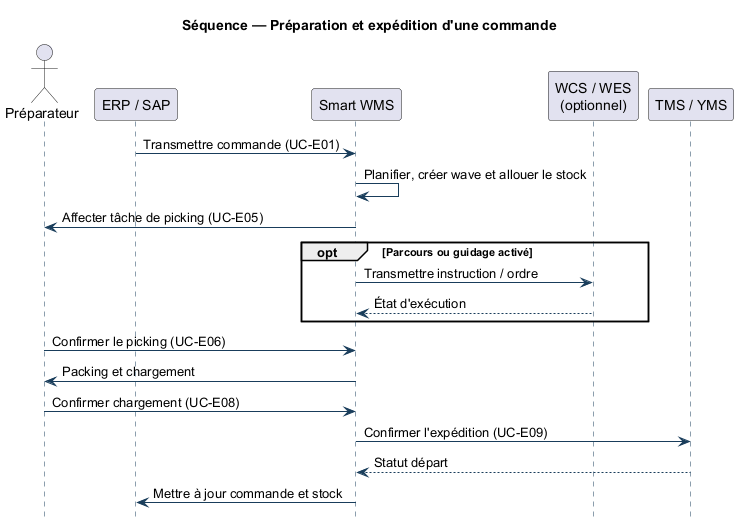
\includegraphics[width=.96\linewidth,height=.78\textheight,keepaspectratio]{figures/uml/seq_expedition.png}
\caption{Diagramme de séquence de la préparation et de l'expédition.}
\label{fig:sequence-expedition}
\end{figure}
\FloatBarrier

\section{Modèle de domaine}
\label{sec:5.5}

Le modèle de domaine identifie les entités utilisées de manière récurrente par les processus : produit, unité logistique, lot, stock, emplacement, zone, tâche, opérateur, équipement, mesure, alerte et recommandation. Il permet de relier les décisions Smart aux objets opérationnels concernés, sans confondre le modèle métier avec une implémentation de base de données.

\begin{figure}[p]
\centering
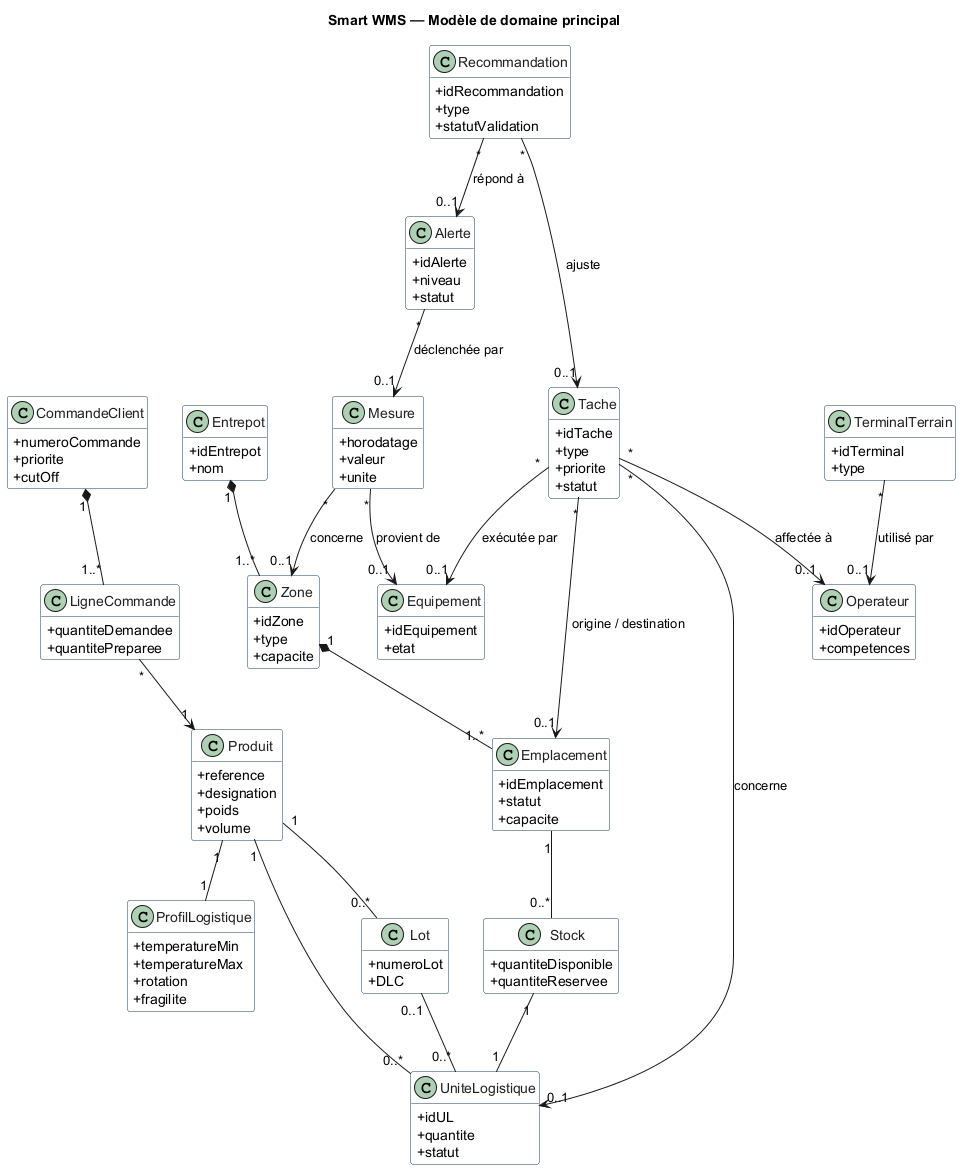
\includegraphics[width=.88\linewidth,height=.84\textheight,keepaspectratio]{figures/uml/modele_domaine.png}
\caption{Modèle de domaine principal du Smart WMS.}
\label{fig:modele-domaine}
\end{figure}
\FloatBarrier

\section{Organisation logique des composants}
\label{sec:5.6}

La vue de composants organise la solution autour des services métier WMS, d'un moteur de tâches, des services Smart, des données, des canaux terrain et des systèmes externes. Cette séparation soutient l'évolution progressive du système : une intégration WCS/WES ou un service de vision peut être ajouté sans modifier la responsabilité des processus 	extit{Core}.

\begin{figure}[p]
\centering
\resizebox{.92\linewidth}{!}{\begin{tikzpicture}[x=1cm,y=1cm,>=Stealth, every node/.style={font=\sffamily\fontsize{8.4}{10}\selectfont,align=center}]
\tikzset{band/.style={draw=Navy,line width=.55pt,rounded corners=1pt}, cell/.style={draw=Navy!70,fill=white,line width=.45pt,minimum height=1.0cm,inner sep=2pt}, arrow/.style={->,draw=Navy,line width=.55pt}}
\node[band,fill=Teal!8,minimum width=15.8cm,minimum height=2.0cm,anchor=north west] (terrain) at (0,22) {};
\node[anchor=north west,font=\sffamily\bfseries\fontsize{10}{12}\selectfont,text=Teal] at (.25,21.75) {Canaux et terrain};
\node[cell,minimum width=4.4cm] (vision) at (3,20.75) {Lecture et vision\\RFID, OCR, caméra};
\node[cell,minimum width=4.4cm] (term) at (8,20.75) {Terminaux RF / mobiles};
\node[cell,minimum width=4.4cm] (equip) at (13,20.75) {Équipements\\AMR, convoyeurs, AS/RS};

\node[band,fill=Orange!9,minimum width=15.8cm,minimum height=2.0cm,anchor=north west] (ext) at (0,19.35) {};
\node[anchor=north west,font=\sffamily\bfseries\fontsize{10}{12}\selectfont,text=Orange] at (.25,19.10) {Systèmes externes};
\node[cell,minimum width=3.1cm] (erp) at (2,18.1) {ERP / SAP};
\node[cell,minimum width=3.1cm] (tms) at (5.55,18.1) {TMS / YMS};
\node[cell,minimum width=3.1cm] (wcs) at (9.10,18.1) {WCS / WES};
\node[cell,minimum width=3.1cm] (bms) at (12.65,18.1) {BMS / EMS};

\node[band,fill=Navy!7,minimum width=15.8cm,minimum height=5.1cm,anchor=north west] (wms) at (0,16.7) {};
\node[anchor=north west,font=\sffamily\bfseries\fontsize{10}{12}\selectfont,text=Navy] at (.25,16.45) {Services métier WMS};
\node[cell,minimum width=4.6cm] (rec) at (2.7,15.25) {Réception};
\node[cell,minimum width=4.6cm] (stock) at (8,15.25) {Stockage et inventaire};
\node[cell,minimum width=4.6cm] (exp) at (13.3,15.25) {Commandes et expédition};
\node[cell,minimum width=4.6cm] (yard) at (2.7,13.65) {Yard et quais};
\node[cell,minimum width=4.6cm] (res) at (8,13.65) {Ressources et actifs};
\node[cell,fill=Navy!12,minimum width=4.6cm] (tasks) at (13.3,13.65) {Moteur de tâches};

\node[band,fill=Purple!8,minimum width=15.8cm,minimum height=2.5cm,anchor=north west] (smart) at (0,10.85) {};
\node[anchor=north west,font=\sffamily\bfseries\fontsize{10}{12}\selectfont,text=Purple] at (.25,10.60) {Services Smart};
\node[cell,minimum width=4.6cm] (optim) at (2.7,9.45) {Prévision et optimisation};
\node[cell,minimum width=4.6cm] (anomaly) at (8,9.45) {Détection d'anomalies};
\node[cell,minimum width=4.6cm] (rules) at (13.3,9.45) {Règles et recommandations};

\node[band,fill=Purple!4,minimum width=15.8cm,minimum height=3.6cm,anchor=north west] (data) at (0,7.65) {};
\node[anchor=north west,font=\sffamily\bfseries\fontsize{10}{12}\selectfont,text=Purple] at (.25,7.40) {Données};
\node[cell,minimum width=4.6cm] (ref) at (2.7,6.15) {Référentiel métier};
\node[cell,minimum width=4.6cm] (oltp) at (8,6.15) {Base opérationnelle\\OLTP};
\node[cell,minimum width=4.6cm] (dwh) at (13.3,6.15) {Entrepôt analytique\\OLAP / DWH};

\draw[arrow] (vision.south) -- (rec.north);
\draw[arrow] (term.south) -- (tasks.north);
\draw[arrow] (equip.south) -- (wcs.north);
\draw[arrow] (erp.south) -- (rec.north);
\draw[arrow] (tms.south) -- (exp.north);
\draw[arrow] (wcs.south) -- (tasks.north);
\draw[arrow] (bms.south) -- (anomaly.north);
\draw[arrow] (rec.south) -- (tasks.north west);
\draw[arrow] (stock.south) -- (tasks.north west);
\draw[arrow] (exp.south) -- (tasks.north);
\draw[arrow] (yard.south) -- (tasks.west);
\draw[arrow] (res.south) -- (tasks.west);
\draw[arrow] (ref.south) -- (oltp.south);
\draw[arrow] (oltp.east) -- (dwh.west);
\draw[arrow] (dwh.north) -- (optim.south);
\draw[arrow] (dwh.north) -- (anomaly.south);
\draw[arrow] (optim.east) -- (rules.west);
\draw[arrow] (anomaly.east) -- (rules.west);
\draw[arrow] (rules.north) -- node[right,font=\sffamily\fontsize{7}{8}\selectfont]{recommandation validée} (tasks.south);
\end{tikzpicture}
}
\caption{Organisation logique des composants du Smart WMS.}
\label{fig:composants}
\end{figure}
\FloatBarrier

\section{Synthèse du chapitre}
\label{sec:5.7}

La modélisation UML confirme la cohérence entre les besoins, les cas d'utilisation et l'architecture fonctionnelle. Elle rend la modularité vérifiable : les processus essentiels demeurent disponibles dans le socle 	extit{Core}, les décisions enrichies relèvent du niveau 	extit{Smart} et les capacités dépendantes d'un équipement restent 	extit{Optional}. Les modèles produits constituent ainsi une base de conception et de discussion pour une future architecture applicative, sans présumer d'un choix technologique ou d'une implémentation particulière.
